\documentclass{oblivoir}
\usepackage{amsmath,amssymb,amsthm,kotex,paralist,kswrapfig}

\usepackage[skipabove=10pt]{mdframed}

\usepackage{tabto,pifont}
\TabPositions{0.2\textwidth,0.4\textwidth,0.6\textwidth,0.8\textwidth}
\newcommand\tabb[5]{\par\bigskip\noindent
\ding{172}\:{\ensuremath{#1}}
\tab\ding{173}\:\:{\ensuremath{#2}}
\tab\ding{174}\:\:{\ensuremath{#3}}
\tab\ding{175}\:\:{\ensuremath{#4}}
\tab\ding{176}\:\:{\ensuremath{#5}}}

\usepackage{enumitem}
%\setlist{noitemsep}
\setlist[enumerate]{label=(\arabic*)}

\newcounter{num}
\newcommand{\prob}[1]
{\bigskip\noindent\refstepcounter{num}\textbf{문제 \arabic{num}) #1}\par\noindent}

\newcommand{\ans}{
{\par
\raggedleft\textbf{답 : (\qquad\qquad\qquad\qquad\qquad\qquad)}
\par}\bigskip\bigskip}

\newcommand\ov[2]{\ensuremath{\overline{#1#2}}}

\newcommand{\pa}{\mathbin{\:\!/\mkern-5mu/\!\:}}

%\newcommand{\pb}[1]%\Phantom + fBox
%{\fbox{\phantom{\ensuremath{#1}}}}

%%%%
\begin{document}

\title{윤영 : 04 쎈(2)}
\author{}
\date{\today}
\maketitle

\setcounter{section}{18}
%%
\section{원과 직선}

%
\prob{855}
\kswrapfig[Pos=r,Width=4cm]{855}{
오른쪽 그림과 같이 지름의 길이가 \(30\)cm인 원 \(O\)에서 \ov AB=\ov CD=\(24\)cm, \(\ov AB\pa \ov CD\)일 때, 두 현 \(AB\), \(CD\) 사이의 거리를 구하여라.
}

\tabb6789{10}

%%
%\prob{860a}
%오른쪽 그림과 같이 \(\triangle ABC\)의 외접원의 중심 \(O\)에서 세 변 \(AB\), \(BC\), \(CA\)에 내린 수선의 발을 각각 \(D\), \(E\), \(F\)라고 하자.
%\(\ov OD=\ov OE=\ov OF\)이고, \(\ov AB=6\)cm일 때, 원 \(O\)의 넓이를 구하여라.

%
\prob{860}
\kswrapfig[Pos=r,Width=4cm]{860}{
오른쪽 그림과 같이 육각형 \(ABCDEF\)의 외접원의 중심 \(O\)에서 여섯 변 \(AB\), \(BC\), \(CD\), \(DE\), \(EF\), \(FA\)에 내린 수선의 발을 각각 \(G\), \(H\), \(I\), \(J\), \(K\), \(L\)이라고 하자.
\(\ov OG=\ov OH=\ov OI=\ov OJ=\ov OK=\ov OL\)이고, \(\ov CI=2\)cm일 때, 원 \(O\)의 넓이를 구하여라.
}
\tabb{15\pi}{16\pi}{17\pi}{18\pi}{19\pi}

%
\prob{881a}
\kswrapfig[Pos=r,Width=3cm]{881a}{
오른쪽 그림과 같이 점 \(A\)에서 원 \(O\)에 그은 두 접선의 접점을 \(E\), \(F\)라고 하자.
\ov BC가 원 \(O\)와 접하고, \(\angle EAF=90^\circ\), \ov AO=\(8\)cm일 때, \(\triangle ABC\)의 둘레의 길이를 구하여라.
}
\tabb{4}{4\sqrt2}{4\sqrt3}{8}{8\sqrt2}

%
\prob{881b}
\kswrapfig[Pos=r,Width=5cm]{881b}{
오른쪽 그림과 같이 점 \(A\)에서 원 \(O\)에 그은 두 접선의 접점을 \(E\), \(F\)라고 하자.
\ov BC가 원 \(O\)와 접하고, \(\angle EAF=120^\circ\), \ov AO=\(8\)cm일 때, \(\triangle ABC\)의 둘레의 길이를 구하여라.
}
\tabb{4}{4\sqrt2}{4\sqrt3}{8}{8\sqrt2}

%
\prob{888}
\kswrapfig[Pos=r,Width=5cm]{888}{
오른쪽 그림과 같이 반원 \(O\)의 지름의 양 끝 점 \(A\), \(B\)에서 그은 접선과 원 위의 점 \(P\)에서 그은 접선이 만나는 점을 각각 \(C\), \(D\)라고 하자.
\ov AC=5cm, \ov BD=3cm일 때, \(\triangle COD\)의 넓이를 구하여라.
}
\tabb{8\sqrt{13}}{8\sqrt{14}}{8\sqrt{15}}{32}{8\sqrt{17}}

%
\prob{900}
\kswrapfig[Pos=r,Width=4cm]{900}{
오른쪽 그림과 같이 \(\angle A=90^\circ\)인 직각삼각형 \(ABC\)의 외접원의 반지름의 길이는 \(13\), 내접원의 반지름의 길이는 \(4\)이다.
이때 \(\triangle ABC\)의 넓이를 구하여라.
}
\tabb{30}{60}{90}{120}{150}

%세로 6, 가로 10
\prob{914}
\kswrapfig[Pos=r,Width=4cm]{914}{
오른쪽 그림과 같은 직사각형 \(ABCD\)의 점 \(B\)를 중심으로 점 \(A\)를 지나는 사분원을 그린 후 점 \(C\)에서 이 원에 접선을 그어 원과의 접점을 \(E\), \ov AD와 만나는 점을 \(F\)라고 하자.
이때 \ov AF의 길이를 구하여라.
}
\tabb{0.5\text{cm}}{1\text{cm}}{1.5\text{cm}}{2\text{cm}}{2.5\text{cm}}

%
\prob{917}
\kswrapfig[Pos=r,Width=4cm]{917}{
오른쪽 그림과 같이 반지름의 길이가 2cm, 중심각의 크기가 \(90^\circ\)인 부채꼴 \(AOB\)에 내접하는 원 \(O'\)의 넓이는?
}
\tabb{4(3-2\sqrt2)\pi\text{cm}^2}{8(3-2\sqrt2)\pi\text{cm}^2}{16(3-2\sqrt2)\pi\text{cm}^2}{4(2\sqrt2-1)\pi\text{cm}^2}{8(2\sqrt2-1)\pi\text{cm}^2}

%
\prob{918a}
\kswrapfig[Pos=r,Width=4cm]{918a}{
오른쪽 그림과 같이 두 원 \(O\), \(O'\)이 서로 외접하고 두 원의 공통인 접선의 교점을 \(P\), 한 접선과 두 원 \(O\), \(O'\)의 접점을 각각 \(A\), \(B\)라고 하자.
\ov PA=2cm, \ov AB=4cm일 때, 원 \(O\)의 반지름의 길이를 구하여라.
}
\tabb{\frac16\sqrt3}{\frac13\sqrt3}{\frac12\sqrt3}{\frac23\sqrt3}{\frac56\sqrt3}

%
\prob{918b}
\kswrapfig[Pos=r,Width=5cm]{918b}{
오른쪽 그림과 같이 두 원 \(O\), \(O'\)이 서로 외접하고 두 원의 공통인 접선의 교점을 \(P\), 한 접선과 두 원 \(O\), \(O'\)의 접점을 각각 \(A\), \(B\)라고 하자.
\ov PA=4cm, \ov AB=2cm일 때, 원 \(O\)의 반지름의 길이를 구하여라.
}
\tabb{\frac{\sqrt2}6}{\frac{\sqrt3}6}{\frac23}{\frac{\sqrt5}6}{\frac{\sqrt6}6}

%
\prob{919}
\kswrapfig[Pos=r,Width=3.5cm]{919}{
오른쪽 그림에서 원 \(O\)는 \(\ov AC=4\sqrt2\)cm, \(\ov AB=\ov BC=2\sqrt3\)cm인 이등변삼각형 \(ABC\)의 외접원일 때, 원 \(O\)의 넓이는?
}
\tabb{5\pi\text{cm}^2}{6\pi\text{cm}^2}{7\pi\text{cm}^2}{8\pi\text{cm}^2}{9\pi\text{cm}^2}

%
\prob{928a}
\kswrapfig[Pos=r,Width=4cm]{928a}{
오른쪽 그림과 같이 원 \(O\)의 지름의 양 끝점 \(A\), \(B\)에서 그은 두 접선과 원 위의 한 점 \(P\)에서 그은 접선이 만나는 점을 각각 \(C\), \(D\)라고 하고 \ov AD와 \ov BC의 교점을 \(Q\)라고 하자.
이때 \ov PQ의 길이를 구하여라.
}
\tabb{\frac{12}7}{\frac{13}7}{2}{\frac{15}7}{\frac{16}7}

%
\prob{928b}
\kswrapfig[Pos=r,Width=4cm]{928b}{
오른쪽 그림과 같이 원 \(O\)의 지름의 양 끝점 \(A\), \(B\)에서 그은 두 접선과 원 위의 한 점 \(P\)에서 그은 접선이 만나는 점을 각각 \(C\), \(D\)라고 하고 \ov AD와 \ov BC의 교점을 \(Q\)라고 하자.
이때 \(\triangle CPQ\)의 둘레의 길이를 구하여라.
}
\tabb{\frac{3+\sqrt{13}}2}{\frac{4+\sqrt{13}}2}{\frac{5+\sqrt{13}}2}{\frac{6+\sqrt{13}}2}{\frac{7+\sqrt{13}}2}

%
\prob{929}
\kswrapfig[Pos=r,Width=4cm]{929}{
오른쪽 그림과 같이 중심이 같은 두 원이 있다.
색칠한 부분의 넓이가 \(16\pi\text{cm}^\circ\)일 때, 작은 원에 접하는 현 \(AB\)의 길이는?
}
\tabb{4}{\sqrt{17}}{2\sqrt{3}}{\sqrt{19}}{2\sqrt5}

%
\prob{932}
\kswrapfig[Pos=r,Width=5cm]{932}{
오른쪽 그림과 같이 반원 \(O\)는 \(\angle A=90^\circ\)인 직각삼각형 \(ABC\)의 빗변 \(BC\)위에 중심이 있고, \ov AB, \ov AC와 각각 점 \(D\), \(E\)에서 접한다.
이때 반원 \(O\)의 반지름의 길이를 구하여라.
}
\tabb{\frac{30}{17}}{\frac{45}{17}}{\frac{60}{17}}{\frac{75}{17}}{\frac{90}{17}}

%
\prob{933}
\kswrapfig[Pos=r,Width=5cm]{933}{
오른쪽 그림과 같은 직사각형 \(ABCD\)의 둘레의 길이는 34cm이고, 두 원 \(O\), \(O'\)은 각각 \(\triangle ABC\), \(\triangle ACD\)의 내접원이다.
두 원의 반지름의 길이가 \(2\)cm로 같고 점 \(E\), \(F\), \(G\), \(H\)는 접점일 때, \(\square GOHO'\)의 넓이는?
}
\tabb{10}{12}{14}{16}{18}

%
\prob{934}
\kswrapfig[Pos=r,Width=4cm]{934}{
\(\square ABCD\)가 원 \(O\)에 외접하고 두 대각선이 직교한다. \ov BC=5, \ov CD=3일 때, \(xy\)의 값을 구하여라.
}
\tabb{6}{9}{15}{18}{21}

%
\prob{935}
\kswrapfig[Pos=r,Width=4cm]{935}{
오른쪽 그림과 같이 두 원 \(P\), \(Q\)는 서로 외접하고 동시에 지름의 길이가 \(6\)인 반원 \(O\)에 내접한다.
이떄, 원 \(Q\)의 둘레의 길이를 구하여라.
}
\tabb{\pi}{2\pi}{3\pi}{4\pi}{5\pi}

%
\prob{936}
반지름의 길이가 \(12\)인 원의 일부인 부채꼴 \(OAB\)로 원뿔을 만들었더니 밑면의 반지름의 길이가 \(4\)이었다.
원의 중심 \(O\)에서 현 \(AB\)까지의 거리를 구하여라.
\begin{figure}[h!]
\centering
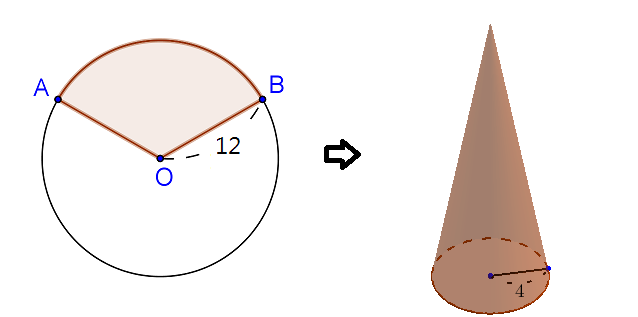
\includegraphics[width=0.5\textwidth]{936completed}
\end{figure}
\tabb2468{10}

%
\prob{940}
\kswrapfig[Pos=r,Width=4cm]{940}{
오른쪽 그림에서 \(\square ABCD\)는 \ov AB=4, \ov BC=3인 직사각형이다.
\ov BE가 \ov CD를 지름으로 하는 반원에 접할 때, \ov BE의 길이를 구하여라.
}
\tabb{\frac{10}3}{\frac{11}3}4{\frac{13}3}{\frac{14}3}

%%
%\prob{944}
%\kswrapfig[Pos=r,Width=4cm]{944}{
%오른쪽 그림과 같이 \(\angle A=\angle B=90^\circ\)인 사다리꼴 \(ABCD\)에 원 \(O\)가 내접하고 있을 때, 색칠한 부분의 넓이를 구하여라.
%}

%
\prob{946a}
\kswrapfig[Pos=r,Width=4cm]{946a}{
오른쪽 그림과 같이 원 \(O'\)이 반지름의 길이가 \(15\)cm인 부채꼴 \(AOB\)에 내접한다.
\(\angle AOB=60^\circ\)일 때, 원 \(O'\)의 넓이를 구하여라.
}
\tabb{9\pi}{16\pi}{25\pi}{36\pi}{49\pi}

%
\prob{946b}
\kswrapfig[Pos=r,Width=5cm]{946b}{
오른쪽 그림과 같이 원 \(O'\)이 반지름의 길이가 \(6\)cm인 부채꼴 \(AOB\)에 내접한다.
\(\angle AOB=120^\circ\)일 때, 원 \(O'\)의 넓이를 구하여라.
}
\tabb{32(7-4\sqrt3)\pi}{32(7+4\sqrt3)\pi}{64(7-4\sqrt3)\pi}{64(7+4\sqrt3)\pi}{96(7-4\sqrt3)\pi}

\end{document}